\documentclass[letterpaper]{article}

\usepackage{incertia}[cd]
\usetikzlibrary{arrows}

% setup the header
\pagestyle{fancy}
\lhead{Will Song}
\chead{Burnside's Lemma}
\rhead{AIME Seminar}

\begin{document}
\section{Introduction}
In this lesson we present a wild new (not really) idea to count the number of
configurations that are distinct up to some sort of symmetry.  For example, how
many ways are there to color an $8 \times 8$ board with $4$ colors such that if
you can rotate one configuration $\mathcal{C}_1$ to obtain $\mathcal{C}_2$,
these configurations are considered identical?

To do so, we are going to introduce some machinery and present things in an
abstract manner before moving to the concrete.

\section{Definitions}
\begin{df}
A \textbf{group} $G$ is a set endowed with an associative binary operation $* :
G \times G \to G$ such that the following properties hold.
\begin{enumerate}
\item
$\exists e \in G \st g * e = g = e * g \quad \forall g \in G$.
\item
$\forall g \in G, \exists g^{-1} \in G \st g * g^{-1} = e = g^{-1} * g$.
\end{enumerate}
\end{df}

\begin{rem}
Associativity can be rephrased in the following commutative diagram.
\begin{center}
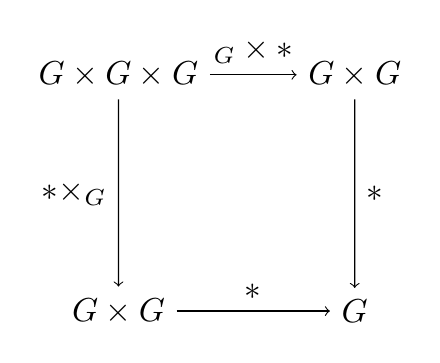
\begin{tikzpicture}[scale=3, nodes={scale=1.2}]
\node (GGG) at (0, 1) {$G \times G \times G$};
\node (GG1) at (1, 1) {$G \times G$};
\node (GG2) at (0, 0) {$G \times G$};
\node (G)   at (1, 0) {$G$};

\path[->]
(GGG) edge node[above]{$\id_G \times *$} (GG1)
(GGG) edge node[left] {$* \times \id_G$} (GG2)
(GG2) edge node[above]{$*$}              (G)
(GG1) edge node[right]{$*$}              (G);
\end{tikzpicture}
\end{center}
\end{rem}

\begin{ex}
$\ZZ, \QQ, \RR, \CC$ under $+$ are groups.
\end{ex}

\begin{ex}
$\QQ^\times, \RR^\times, \CC^\times$ under $\cdot$ are also groups.
\end{ex}

\begin{ex}
The set of rotations of a square under composition form a group.
\end{ex}

\begin{ex}
$\Aut(X)$, the set of bijections from a set $X$ to itself under composition is a
group.
\end{ex}

This is all nice and easy, but groups can so far only talk to themselves. Here
is how groups talk to sets.

\begin{df}
A group $G$ is said to \textbf{act} on a set $X$ if there is a function $\rho :
G \times X \to X$, notated $g \cdot x = \rho(g, x)$, such that the following
properties hold.
\begin{enumerate}
\item
$\rho(1, x) = x \quad \forall x \in X$.
\item
$g \cdot (h \cdot x) = (g * h) \cdot x \quad \forall x \in X, g, h \in G$.
\end{enumerate}
\end{df}

\begin{df}
The \textbf{orbit} of an element $x \in X$ with respect to an action $\rho$ is
the set of all outputs of the action through $\rho$ by holding $x$ constant. In
other words,
\[ Gx = G \cdot x = \orb(x) = \lbrace g \cdot x \mid g \in G \rbrace. \]
\end{df}

\begin{df}
The \textbf{stabilizer} of an element $x \in X$ with respect to an action $\rho$
is the set of all elements in $G$ that do not change $x$, or \textbf{fixes} $x$.
This is notated
\[ G_x = \stab(x) = \lbrace g \in G \mid g \cdot x = x \rbrace. \]
\end{df}

\begin{df}
Denote the elements of $X$ fixed by some $g \in G$ to be
\[ X_g = \fix(g) = \lbrace x \in X \mid g \cdot x = x \rbrace. \]
\end{df}

\begin{ex}
$G$ acts on itself in two important ways. One is left multiplication $g \cdot h
= g * h$. The other is conjugation $g \cdot h = ghg^{-1}$.
\end{ex}

\begin{ex}
Permutations on the set $[1..n]$ act on the set $[1..n]$. For example, $\sigma
\in S_n = \Aut([1..n])$ acts on $[1..n]$ by $\sigma \cdot x = \sigma(x)$.
\end{ex}

\section{Actual Things}
The main result depends on a result called the orbit stabilizer theorem.  We
don't have the machinery of quotient groups yet so I will just state the theorem
and use it.

\begin{thm}[Orbit Stabilizer]
Let finite group $G$ act on $X$. Then
\[ \lvert G \rvert = \lvert G_x \rvert \lvert G \cdot x \rvert \quad \forall x
\in X \]
\end{thm}

We now have a basic understanding of what we need to get Burnside's Lemma.

\begin{lem}[Burnside's Lemma]
Let $G$ be a finite group that acts on finite set $X$. Let $GX = \lbrace Gx \mid
x \in X \rbrace$, or the set of orbits of elements in $X$ via $G$. Then
\[ \lvert GX \rvert \lvert G \rvert = \sum_{g \in G} \lvert X_g \rvert.  \]
In other words, the number of distinct orbits is the average of the number of
elements in $X$ fixed by elements in $G$.
\end{lem}

\begin{proof}
We look at the right hand side and count it in two different ways. Namely,
\[ \sum_{g \in G} \lvert X_g \rvert = \lvert \lbrace (g, x) \in G \times X \mid
g \cdot x = x \rbrace \rvert = \sum_{x \in X} \lvert G_x \rvert \]
Now notice that if $x \in Gy$, then $Gx = Gy$ so $\lvert G_x \rvert = \lvert G_y
\rvert$ by the orbit stabilizer theorem. $X$ is finite so there are a finite
number of orbits so we can sum over representative elements of each orbit to get
\[ \sum_{g \in G} \lvert X_g \rvert = \sum_{i = 1}^{\lvert GX \rvert} \sum_{x
\in Gx_i} \lvert G_x \rvert = \sum_{i = 1}^{\lvert GX \rvert} \lvert Gx_i \rvert
\lvert G_{x_i} \rvert, \]
but the summand is equal to $\lvert G \rvert$ by the orbit stabilzer theorem so
this is just $\lvert GX \rvert \lvert G \rvert$ as desired.
\end{proof}

\subsection{Examples}

\begin{ex}
$5$ people sit in a circle. How many unique seatings are there disregarding
rotations?
\end{ex}

\begin{proof}[Solution]
The beginning combinatorial student will argue that you fix the first person and
there are $4! = 24$ ways of ordering the rest of them. But we are smarter and we
use Burnside's Lemma. The $5$ symmetries we need to count here are \{do nothing,
rotate 1 person, rotate 2 people, rotate 3 people, rotate 4 people\}. Doing
nothing fixes everything and everybody is unique so rotate $n$ people all fix
$0$ arrangements so the number of distinct seatings is $\frac{5! + 0 + 0 + 0 +
0}{5} = 24$.
\end{proof}

\begin{ex}
Compute the number of unique necklaces that can be made from $3$ white beads and
$3$ black beads. Necklaces are unique with respect to rotations and reflections.
\end{ex}

\begin{proof}[Solution]
Again we enumerate the symmetries and compute the number of elements they fix.
As always, the identity fixes $\binom{6}{3} = 20$ elements.  Rotating an odd
number of time trivially fixes $0$ elements, but rotation $2$ or $4$ times each
fix $2$ elements. Reflections through midpoints fix $0$ elements because the
side that has even blacks and odd whites goes to the other side. Reflections
through vertices however, fix $4$ elements each (see if you can count this
yourself!), so the number of distinct necklaces is then $\frac{20 + 3 \cdot 0 +
2 \cdot 2 + 3 \cdot 0 + 3 \cdot 4}{12} = \frac{36}{12} = 3$. In fact, it is easy
to find these neclackes as well. They are \{BBBWWW, BBWBWW, BWBWBW\}.
\end{proof}

\subsection{Problems}

\begin{prb}
How many subsets $\lbrace x, y, z, t \rbrace \subset \NN$ satisfy $12 \leq x < y
< z < t$ and $x + y + z + t = 2018$.
\end{prb}

\begin{prb}[1996 AIME]
Two squares of a $7 \times 7$ checkerboard are painted yellow and the rest
green. Two paintings are equivalent if one can be obtained by applying a
rotation to the other. How many inequivalent color schemes are there?
\end{prb}

\begin{prb}[2010 AIME II-10]
Find the number of second degree polynomials $f(x)$ with integer coefficients
and integer zeroes for which $f(0) = 2010$.
\end{prb}

\begin{prb}[2010 AMC 12A-25]
Two quadrilaterals are considered equivalent if one can be obtained by applying
a rotation and or a translation to the other. How many different convex cyclic
quadrilaterals are there with integer side lengths and perimeter $32$?
\end{prb}

\end{document}
